This section presents the results obtained by coding the messages with codes having the same constraint length (in our case, 4) but different code rates. All the three figures (figures \ref{fig:constantContraintRandomFigure}, \ref{fig:constantContraintRandomFigure}, \ref{fig:constantContraintMarkovFigure}) show the same result - the error correction capabilities are better when the code rate is lower. This is due to the fact that more redundancy is added to each message. As opposed to varying the constraint length, the variations in code rate have a straight forward result.

\begin{figure}
\centering
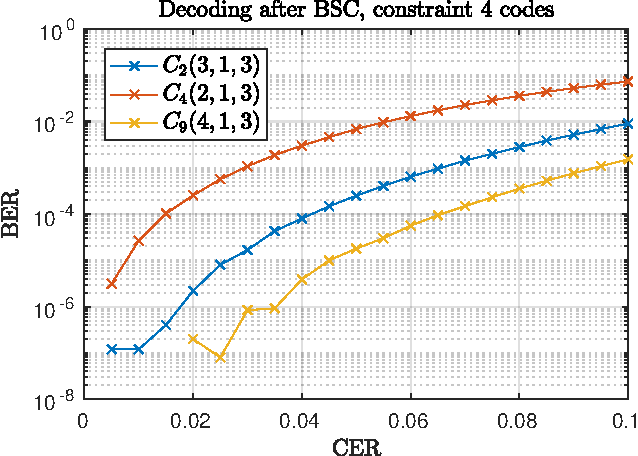
\includegraphics[scale=1]{../figures/const4rand.pdf} 
\caption{Length 4\todo[inline]{change caption}\label{fig:constantContraintRandomFigure}}
\end{figure}

\begin{figure}
\centering
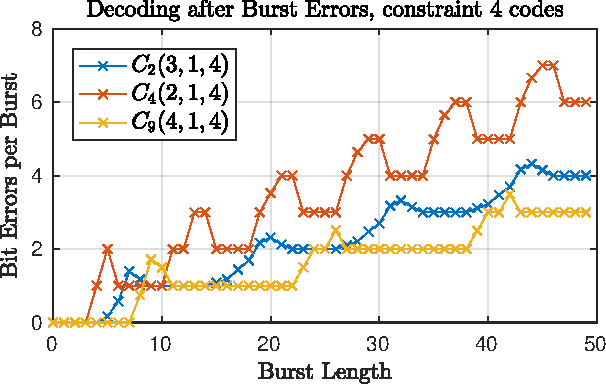
\includegraphics[scale=1]{../figures/const4burst.pdf} 
\caption{Length 4\todo[inline]{change caption}\label{fig:constantContraintBurstFigure}}	
\end{figure}

\begin{figure}
\centering
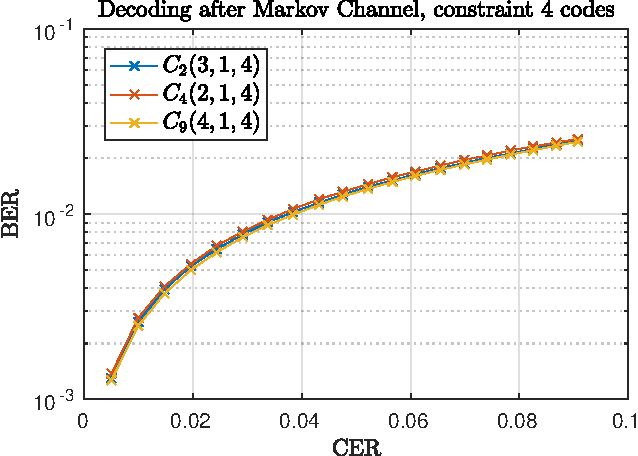
\includegraphics[scale=1]{../figures/const4markov.pdf} 
\caption{Length 4\todo[inline]{change caption}\label{fig:constantContraintMarkovFigure}}
\end{figure}